%\documentclass{article}
%\usepackage[utf8]{inputenc}

\documentclass[12pt]{article}
\usepackage{graphicx} % This lets you include figures
% This lets you make links to web locations

\usepackage[colorlinks=true,linkcolor=blue,urlcolor=blue]{hyperref} 
\graphicspath{ {./images/} }

\usepackage[rightcaption]{sidecap}
\usepackage{subcaption}
\usepackage{wrapfig}
\usepackage{amssymb}
\usepackage{float}
\usepackage{amsmath}
\usepackage{imakeidx}

% Commands created by Sparsh

\let\oldref\ref
\renewcommand{\ref}[1]{(\oldref{#1})}
\renewcommand{\vec}[1]{\mathbf{#1}}

% END Commands created by Sparsh

\makeindex


\title{Tropidance : Trajectory Optimization and Guidance}
\author{Sparsh Yadav}
\date{\today}

\begin{document}
\maketitle{}

\tableofcontents

\clearpage
\newpage

\section{Introduction}

Tropidance is an optimal control toolbox that enables the user to solve challenging trajectory optimization and guidance problems with ease, using direct optimal control techniques. With its ease of use, engineering teams can now get the results to complex optimal control problems rapidly. The potential for the software is limitless and can be used across multiple industries, including aerospace, robotics, energy, mobility and many more. 

Historically, the techniques for solving optimal control problems are broadly classified into direct and indirect methods. Indirect methods rely on the first-order necessary conditions and Pontryagin's minimum principle. These methods lead to a two-point boundary value problem and try to find the optimal trajectories for the state and the control. Although indirect methods enjoy fewer dimensions in the search space, they suffer from extreme sensitivities to the search parameter. The extraordinary speed of modern computers has opened new opportunities for indirect methods for real-time applications. Direct methods transform the optimal control problem into a non-linear constrained optimization problem by discretization of the control input and the system dynamics at finite grid points. Model Predictive Static Programming (MPSP) is one such direct optimal technique.

Optimal control is particularly relevant in Aerospace applications where the economic cost of the mission can be significantly reduced by using optimal control algorithms. The importance of optimal control can be gauged by the fact that, in 2007, using pseudo-spectral optimal control technique  NASA saved 1 million dollars to manoeuvre the International Space Station. It should be noted, the control trajectory was computed offline and uploaded to the International Space station.  Real-time optimal control is still in its nascent stages. To fill the lacuna between offline and real-time applications of optimal control, we need efficient algorithms and faster processors. MPSP has been shown to be computationally efficient for several missile and spacecraft guidance problems. 


\section{Tropidance}

Tropidance builds upon a decade of research into optimal control algorithms for real-time applications. The motivation of the package is to provide researchers, labs, and industry alike, an easy to use, optimal control and guidance software. Anyone with a basic understanding of optimal control should be able to use it without any knowledge of underlying algorithms. The package includes computationally efficient algorithms with mathematically proven convergence properties fit for real-time applications. The software is written in Python, one of the world's most popular programming language, currently implements several state-of-the-art computationally efficient MPSP algorithms developed at ASL, Aerospace Engineering, Indian Institute of Science. The fact it is written in Python makes it platform agnostic, as long as the python interpreter is available, you can get started in less than no time. Tropidance is accompanied with detailed user and developer documentation. The software follows a modular approach and can be extended to implement any number of algorithms.

In summary, Tropidance has the following advantages to the software currently available. Firstly, It implements state-of-the-art MPSP (Model Predictive Static Programming) techniques, which are computationally efficient. Moreover, with several variants of MPSP now available it can address a broad class of optimal control problems. Secondly, It is implemented in Python, an open-source language. Users can quickly get started with the examples provided with the software package with little effort. Thirdly, Tropidance uses open-source libraries and doesn't have a dependency on expensive software like MATLAB, making it more affordable. Finally, the software is built using a modular structure and flexibility in mind; it can be very easily extended to include new algorithms as and when required. The developer documents describe how that can be done.

Numerically, MPSP has the following advantages for solving optimal control problems:
\begin{enumerate}
    \item A dynamic programming problem is converted to a static programming problem, and thus it requires only a static costate vector for the control update
    \item The symbolic costate vector has a closed-form solution for unconstrained problems, which significantly reduces the computational load.
    \item The sensitivity matrices that are necessary to compute the static costate vector are calculated recursively.
\end{enumerate}



\section{Class of problems}

Building on a decade of research, Tropidance implements several MPSP algorithms that have stood the test of time. These algorithms have been extended for several use cases over the years.

\subsection{Fixed Final time $t_f$ with functions of state specified at final time.}

It includes problems in which the functions of the state variables $ \vec{Y} = \vec{H}(\vec{X})$ are prescribed at a fixed terminal time $t_f$. We have system dynmaics given by $\vec{\dot{X}} = \vec{f(X,U)}$ and we want that as $t \rightarrow t_f $, $\vec{Y} \rightarrow \vec{Y^*}$. Several algorithms that can be used to solve such problems include:

% The problem formulation is given in Eq \ref{eq:class1}.

% \begin{equation}
% \begin{aligned}
%     \min_{\vec{U}} \quad & J =  \int_{t_{0}}^{t_{f}} \frac{1}{2} \vec{U}(t)^{\top} \vec{R}  \vec{U}(t) dt\\
%   s.t. \quad & \vec{H}(\vec{X}(t_f))=\vec{Y^*}\\
%   & \vec{U_{lb}} \leqslant \vec{U}(t) \leq \vec{U_{ub}} \quad t \in\left[t_{0}, t_{f}\right] \\
%   & \vec{X}(t_0) = \vec{X_0}
% \end{aligned}
% \label{eq:class1}
% \end{equation}


\subsubsection*{MPSP}
MPSP combines the philosophy of non-linear model predictive control and approximate dynamic programming. The basic version of MPSP is applicable for finite-horizon non-linear problems with terminal constraints was presented in \cite{padhi2009model}. It brings the concept of trajectory optimization into guidance laws which are optimal in regards to the control effort required.

MPSP technique is computationally efficient and can be implemented online, providing for a wide range of real-time applications.  The effectiveness of the method is demonstrated for the ascent phase guidance of a ballistic missile using solid motors in \cite{padhi2009model}.

\subsubsection*{GMPSP}
A generalized version of MPSP was presented in \cite{maity2014generalized} that extends upon the MPSP philosophy for solving a class of finite-horizon non-linear optimal control problems with a hard terminal constraint. Two key features for its high computational efficiency include one-time backward integration of a small-dimensional weighting matrix dynamics, followed by a static optimization formulation that requires only a static Lagrange multiplier to update the control history. Moreover, it turns out that
under Euler integration and rectangular approximation of finite integrals it is equivalent to model predictive static programming technique \cite{padhi2009model}.

\subsubsection*{QS-MPSP}
Quasi-spectral MPSP was proposed in \cite{mondal2018angle} where the control variable is expressed as a weighted sum of basis functions. The coefficients of the basis functions are then determined using optimization techniques, in contrast, to control input at every grid point. This reduces the complexity of the problem and also ensures the smoothness of the control variable. Such a procedure also provides the spread of control over the available time to go.

QS-MPSP guidance was demonstrated in \cite{mondal2018angle} by formulating and solving an angle-constrained missile guidance problem to successfully engage an incoming high-speed ballistic missile target in three dimensions. The proposed QS-MPSP guidance showed considerable improvement in the lateral acceleration demand over the BPN guidance scheme.

\subsection{Tracking Problems}

Trajectory tracking problems can also be solved using the recently developed TMPSP technique.

\subsubsection*{T-MPSP}
A non-linear optimal command tracking technique was presented in \cite{kumar2019model} called the Tracking-oriented MPSP. In this technique, like MPC a model-based prediction-correction approach is adopted.

In \cite{kumar2019model} TMPSP was used for trajectory tracking problem of a two-wheel differential drive mobile robot both in simulations and on real hardware. Successful results in both simulation and hardware implementation study demonstrated that the proposed, computationally efficient, T-MPSP algorithm can be implemented online and is promising for controlling dynamic systems under the paradigm of fast non-linear MPC.

\subsection{Problems with uncertainties in the system parameters}

There are several scenarios where the exact current state of the system can not be deteremined or there are several uncertainities in the system model. In such scenarios recently developed, U-MPSP technique can be used. 

\subsubsection*{U-MPSP}
Unscented MPSP was presented in \cite{mathavaraj2019unscented}, which applies to a class of problems where there are uncertainties in the time-invariant system parameters and/or initial conditions. This technique is a fusion of two recent ideas, namely MPSP and Riemann–Stieltjes optimal control problems. In UMPSP, first an unscented transform is utilized to construct a low-dimensional finite number of deterministic problems. The philosophy of MPSP is utilized next so that the solution can be obtained in a computationally efficient manner. The control solution not only ensures that the terminal constraint is met accurately with respect to the mean value, but it also ensures that the associated covariance matrix (i.e., the error ball) is minimized.

Significance of U-MPSP has been demonstrated in \cite{mathavaraj2019unscented} by successfully solving two benchmark problems, namely the Zermelo problem and inverted pendulum problem, which contain parametric and initial condition uncertainties.


% \subsection{Class 2 : Minimum Final time}

% Class 2 addresses problems in which the functions of state variables $ \vec{Y} = \vec{H}(\vec{X})$ are prescribed at an unspecified final time. The aim is to minimize the time taken to achieve the terminal time boundary conditions. We have system dynmaics given by $\vec{\dot{X}} = \vec{f(X,U)}$ and we want, $\vec{Y} \rightarrow \vec{Y^*}$ in minimum time. The problem formulation is give in Eq \ref{eq:class2}.

% \begin{equation}
% \begin{aligned}
%   \min_{\vec{U}} \quad & J =  \int_{t_{0}}^{t_{f}} dt\\
%   s.t. \quad & \vec{H}(\vec{X}(t_f))=\vec{Y^*}\\
%   & \vec{U_{lb}} \leqslant \vec{U}(t) \leq \vec{U_{ub}} \quad t \in\left[t_{0}, t_{f}\right] \\
%   & \vec{X}(t_0) = \vec{X_0}
% \end{aligned}
% \label{eq:class2}
% \end{equation}


\section{Applications}

Numerous complex engineering problems can be formulated as optimal control or guidance problems, be it guiding a rocket to its desired orbit or optimal guidance for a swarm of drones. Over a decade, the algorithm's feasibility and efficiency have been demonstrated on several benchmarks and engineering problems ranging from biomedical to aerospace applications. 

\begin{itemize}
\item Aerospace : Ascent guidance for rockets, interceptors, and missiles \cite{padhi2009model,dwivedi2011suboptimal,mondal2018angle,oza2012impact,kothari2010nonlinear}; Landing guidance for terrestrial (RLVs) and extra-terrestrial missions \cite{chawla2010suboptimal,Sachan2019,halbe2014robust}; flexible final time guidance \cite{maity2016robust}.
\item Robotics: Trajectory tracking for robotics \cite{kumar2019model} ; Inverted Pendulum \cite{mathavaraj2019unscented}; Unmanned Aerial Systems; Energy sector.
\item Process Control: Biomedical; Industrial Processes etc.
\end{itemize}

\section{Software Architecture}

The aim of the software is usability and extensibility; these principles have been the guiding lights for the development. The software follows a modular approach, with APIs provided to set up and solve the problem. Not only is it user-friendly, but also care has been taken that the software is developer-friendly, and new functionality can be added to the code rapidly.

Tropidance follows a layered architectural pattern with three main layers, namely: 

\begin{itemize}
    \item Client Layer: Contains several client interfaces.
    \item Interface Layer: Provides an abstraction over the core layer so different clients can communicate to the core functionality
    \item Core Layer: Implementation of Algorithms (MPSPS, GMPSP, etc.) and utilities like logging, plotting.
\end{itemize}


The overall block diagram of the package is shown in Figure. \ref{fig:SoftwarePacakgeFlow}.

\begin{figure}[h]
    \centering
    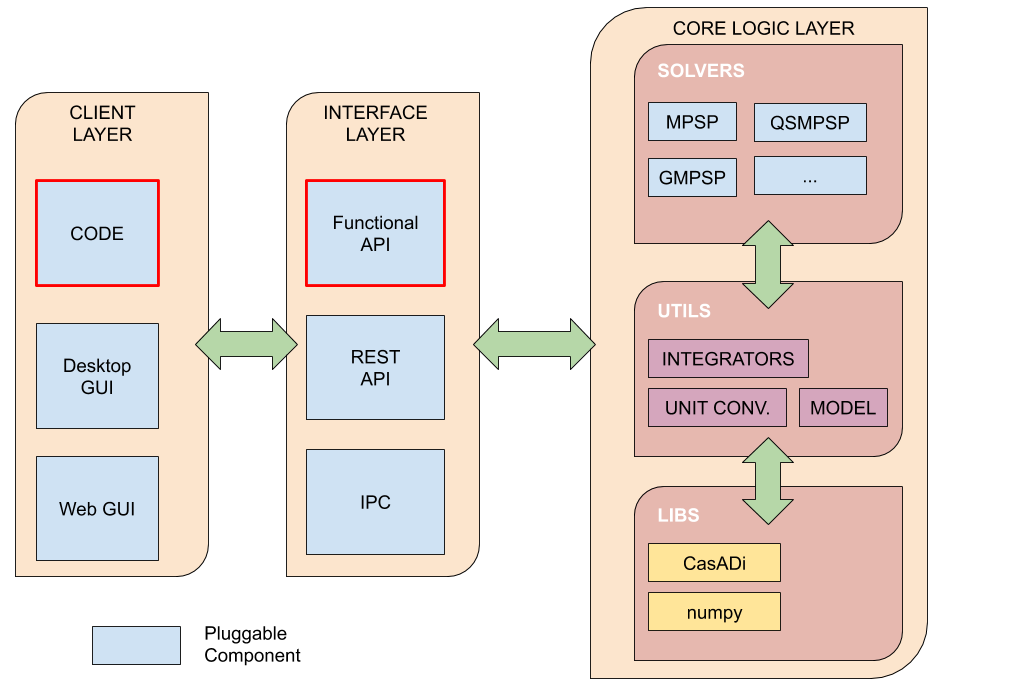
\includegraphics[width=0.9\textwidth]{img/OverallCodeStructure.png}
    \caption{Block diagram of the software package.}
    \label{fig:SoftwarePacakgeFlow}
\end{figure}

\subsection{Python Package}
Tropidance is implemented in Python because of its widespread adoption and ease of use. Moreover, this language is extremely popular with academia and the industry as it a high-level language that enables rapid testing and deployment. The language is also open-source and has a rich collection of scientific libraries.

\subsection{API}
The package provides an easy to use front-end API, which can be used to describe the system dynamics, configure the algorithm and start the solver.

% A sample run is shown in Figure \ref{fig:SampleRun}.

% \begin{figure}[!htb]
%     \centering
%     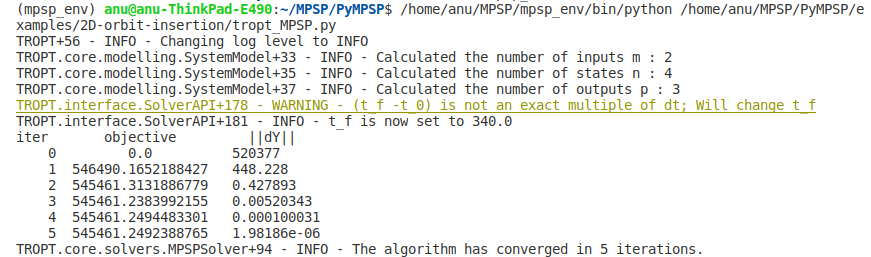
\includegraphics[width=0.9\textwidth]{img/SampleRun.png}
%     \caption{A sample run of the Tropidance package.}
%     \label{fig:SampleRun}
% \end{figure}


\subsection{Salient features of Tropidance}

The software package has several advantages over existing packages which are enumerated below:

\begin{itemize}
\item Configuring the system model is straight-forward.
\item It is easy to configure a particular algorithm and its parameters. 
\item A simple front-end API for the user, that can be used for coding or to create a GUI. 
\item Comes with a logging module that provides verbose and descriptive messages to guide the user and help with debugging.
\item Uses the principles of OOP (Object-oriented programming).
\item Requires no knowledge of underlying algorithms.
\item The aim is to write extensive tests for regression testing. 
\item Thorough documentation autogenerated with pydoc. 
\item Source and version control using git.
\end{itemize}

\bibliographystyle{unsrt}
\bibliography{main}

%\href{http://class.guilford.edu/physics/dasmith}{this way}

%\footnote{You can put the link in a footnote like this.}

% Anything to the right of a percent sign will be ignored by LaTeX.
% You can use this to put notes to yourself.  If you want to actually
% get a percent sign in your PDF file, use \%.  This holds for many 
% symbols, like \$ and \&.  Without the backslash, LaTeX will think
% you are trying to give it a command, and it will get confused.
% Note that this paragraph does not show up in the PDF.

% \listoffigures

\medskip
\end{document}
